\documentclass[aspectratio=169,10pt]{beamer}

\usetheme{Madrid}
\usecolortheme{seahorse}
\setbeamertemplate{navigation symbols}{}
\setbeamertemplate{footline}[frame number]
\setbeamertemplate{caption}[numbered]

\usepackage{amsmath}
\usepackage{amssymb}
\usepackage{booktabs}
\usepackage{graphicx}
\usepackage{mathtools}
\usepackage{array}

\newcommand{\dd}{\,\mathrm{d}}
\newcommand{\ii}{\mathrm{i}}
\newcommand{\eoc}{\mathrm{EOC}}
\newcommand{\norm}[1]{\left\lVert #1\right\rVert}

\title[One-Way Wave Equation]{Finite Difference Methods for the One-Way Wave Equation}
\subtitle{Consistency, convergence, and stability under parameter sweeps}
\author{Rishabh Kumar}
\institute{MH7007 Topics in Scientific Computation I}
\date{\today}

\begin{document}

\begin{frame}
    \titlepage
\end{frame}

\begin{frame}{Problem and Exact Solution}
    We solve the initial-boundary value problem
    \begin{equation}
        u_t+u_x=0,\qquad x>-2,\quad t>0,\qquad u(-2,t)=0,
    \end{equation}
    with compactly supported initial data
    \begin{equation}
        u_0(x)=
        \begin{cases}
            (1-|x|)^2, & |x|\le 1,\\
            0, & |x|>1.
        \end{cases}
    \end{equation}

    Since the speed is $a=1$, characteristics satisfy $x-t=\mathrm{constant}$, so
    \begin{equation}
        u(x,t)=
        \begin{cases}
            u_0(x-t), & x-t\ge -2,\\
            0, & x-t<-2.
        \end{cases}
    \end{equation}

    The left boundary is inflow; the right boundary $x=b$ is outflow.
\end{frame}

\begin{frame}{Grid, Errors, and Sweep Parameters}
    Let
    \begin{equation}
        x_m=-2+mh,\qquad t_n=nk,\qquad
        v_m^n\approx u(x_m,t_n),\qquad \lambda=\frac{k}{h}.
    \end{equation}
    Since the wave speed is $a=1$, $\lambda$ is the Courant number.  Thus
    $\lambda=1$ means that the exact wave travels one grid cell during one time step.

    At a final time $T$, define
    \begin{equation}
        E_1=h\sum_m |v_m^N-u(x_m,T)|,\qquad
        E_2=\left(h\sum_m |v_m^N-u(x_m,T)|^2\right)^{1/2},
    \end{equation}
    \begin{equation}
        E_\infty=\max_m |v_m^N-u(x_m,T)|,\qquad
        \eoc=\frac{\log(E_h/E_{h/2})}{\log 2}.
    \end{equation}

    \begin{block}{Task sweep}
        \[
            b\in\{3,4,5\},\qquad
            h\in\{0.1,0.05,0.01\},\qquad
            \lambda\in\{0.8,0.9,1.0,1.01,1.05,1.1\}.
        \]
    \end{block}
\end{frame}

\begin{frame}{Explicit Schemes}
    With $\nu=a k/h=\lambda$ for this problem, the main explicit updates are
    \scriptsize
    \begin{align}
        \text{FTFS:}\quad
        v_m^{n+1}&=(1+\nu)v_m^n-\nu v_{m+1}^n,\\
        \text{FTBS:}\quad
        v_m^{n+1}&=(1-\nu)v_m^n+\nu v_{m-1}^n,\\
        \text{FTCS:}\quad
        v_m^{n+1}&=v_m^n-\frac{\nu}{2}(v_{m+1}^n-v_{m-1}^n),\\
        \text{CTCS:}\quad
        v_m^{n+1}&=v_m^{n-1}-\nu(v_{m+1}^n-v_{m-1}^n),\\
        \text{Lax--Friedrichs:}\quad
        v_m^{n+1}&=\frac{1+\nu}{2}v_{m-1}^n+\frac{1-\nu}{2}v_{m+1}^n,\\
        \text{Lax--Wendroff:}\quad
        v_m^{n+1}&=v_m^n-\frac{\nu}{2}(v_{m+1}^n-v_{m-1}^n)
        +\frac{\nu^2}{2}(v_{m+1}^n-2v_m^n+v_{m-1}^n).
    \end{align}
    \normalsize
    Beam--Warming uses a one-sided second-order upwind stencil:
    \[
        v_m^{n+1}=v_m^n-\frac{\nu}{2}(3v_m^n-4v_{m-1}^n+v_{m-2}^n)
        +\frac{\nu^2}{2}(v_m^n-2v_{m-1}^n+v_{m-2}^n).
    \]
\end{frame}

\begin{frame}{Implicit Schemes}
    The implicit methods solve a tridiagonal linear system at each time step.
    \small
    \begin{align}
        \text{BTFS:}\quad
        (1-\nu)v_m^{n+1}+\nu v_{m+1}^{n+1}
        &=v_m^n,\\
        \text{BTBS:}\quad
        (1+\nu)v_m^{n+1}-\nu v_{m-1}^{n+1}
        &=v_m^n,\\
        \text{BTCS:}\quad
        v_m^{n+1}
        +\frac{\nu}{2}(v_{m+1}^{n+1}-v_{m-1}^{n+1})
        &=v_m^n,\\
        \text{Crank--Nicolson:}\quad
        v_m^{n+1}
        +\frac{\nu}{4}(v_{m+1}^{n+1}-v_{m-1}^{n+1})
        &=
        v_m^n-\frac{\nu}{4}(v_{m+1}^{n}-v_{m-1}^{n}).
    \end{align}

    \vspace{0.15cm}
    BTBS is the implicit upwind scheme for right-moving advection.  Crank--Nicolson is formally second-order and nondissipative, so it preserves amplitudes well but may retain oscillations near nonsmooth corners.
\end{frame}

\begin{frame}{Formal Accuracy}
    Taylor expansion gives the formal local truncation errors for smooth solutions.

    \begin{table}
        \centering
        \small
        \begin{tabular}{@{}lll@{}}
            \toprule
            Scheme & Local truncation error & Order if $k=O(h)$\\
            \midrule
            FTFS, FTBS & $O(k+h)$ & first\\
            FTCS & $O(k+h^2)$ & first\\
            CTCS & $O(k^2+h^2)$ & second\\
            Lax--Friedrichs & $O(k+h^2/k)$ & first\\
            Lax--Wendroff & $O(k^2+h^2)$ & second\\
            Beam--Warming & $O(k^2+h^2)$ & second\\
            BTFS, BTBS & $O(k+h)$ & first\\
            BTCS & $O(k+h^2)$ & first\\
            Crank--Nicolson & $O(k^2+h^2)$ & second\\
            \bottomrule
        \end{tabular}
    \end{table}

    \begin{alertblock}{Important caveat}
        The assigned $u_0$ is continuous but has a corner at $x=0$.  Therefore max-norm convergence can be lower than the formal smooth-solution order, especially for higher-order dispersive schemes.
    \end{alertblock}
\end{frame}

\begin{frame}{Von Neumann Stability}
    Insert the Fourier mode $v_m^n=G^n e^{\ii m\theta}$ and require $|G(\theta)|\le 1$.

    \begin{table}
        \centering
        \scriptsize
        \begin{tabular}{@{}lll@{}}
            \toprule
            Scheme & Amplification factor & Stable range for $a>0$\\
            \midrule
            FTFS & $1+\nu-\nu e^{\ii\theta}$ & unstable\\
            FTBS & $1-\nu+\nu e^{-\ii\theta}$ & $0\le\nu\le1$\\
            FTCS & $1-\ii\nu\sin\theta$ & unstable\\
            CTCS & $G^2+2\ii\nu\sin\theta\,G-1=0$ & $|\nu|\le1$\\
            Lax--Friedrichs & $\cos\theta-\ii\nu\sin\theta$ & $|\nu|\le1$\\
            Lax--Wendroff & $1-\ii\nu\sin\theta+\nu^2(\cos\theta-1)$ & $|\nu|\le1$\\
            Beam--Warming & second-order upwind symbol & $0\le\nu\le2$\\
            BTBS & $(1+\nu-\nu e^{-\ii\theta})^{-1}$ & all $\nu\ge0$\\
            BTCS & $(1+\ii\nu\sin\theta)^{-1}$ & all $\nu$\\
            Crank--Nicolson & $\dfrac{1-\frac{\ii\nu}{2}\sin\theta}{1+\frac{\ii\nu}{2}\sin\theta}$ & all $\nu$\\
            \bottomrule
        \end{tabular}
    \end{table}

    The experiments below test these theoretical predictions numerically.
\end{frame}

\begin{frame}{Profile Comparison at $\lambda=0.8$}
    \begin{figure}
        \centering
        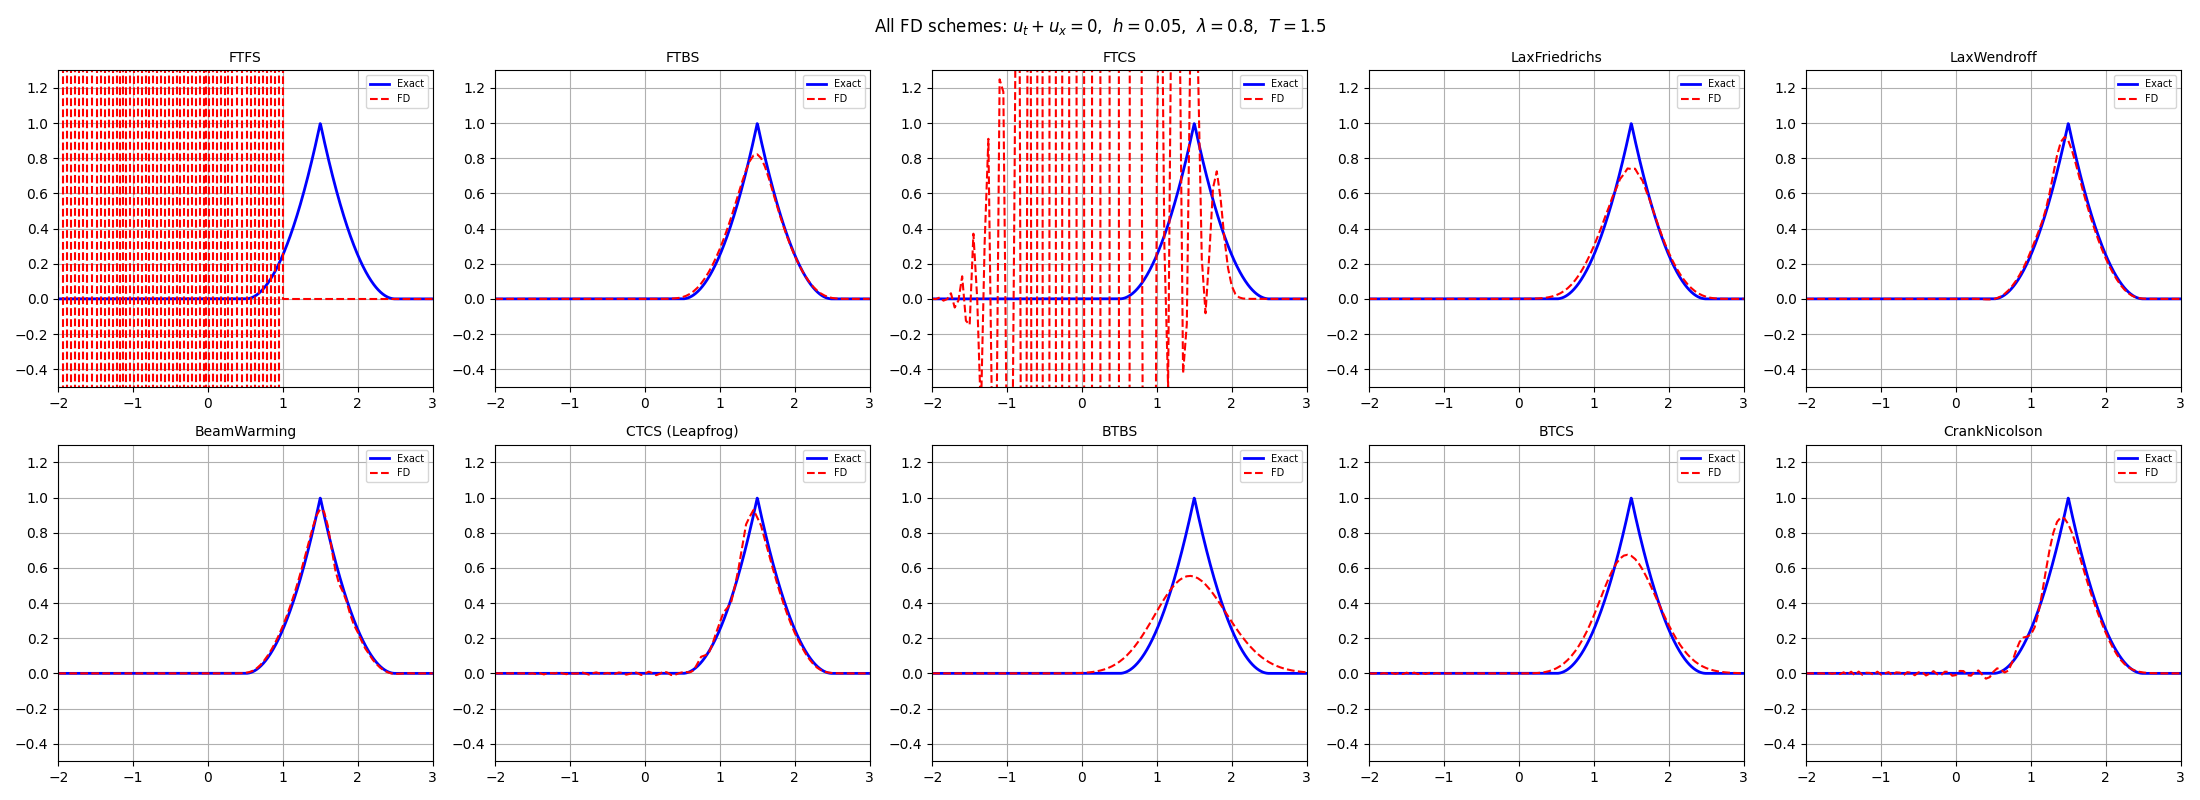
\includegraphics[width=0.88\textwidth]{figures/problem3_all_schemes.png}
    \end{figure}
    \vspace{-0.15cm}
    \small
    At $T=1.5$, $h=0.05$, and $b=3$, the exact pulse has moved to roughly $[0.5,2.5]$.  FTBS and Lax--Friedrichs are stable but diffusive; Lax--Wendroff, CTCS, and Beam--Warming are sharper but more oscillatory near nonsmooth features.
\end{frame}

\begin{frame}{Numerical Convergence Plots}
    \begin{figure}
        \centering
        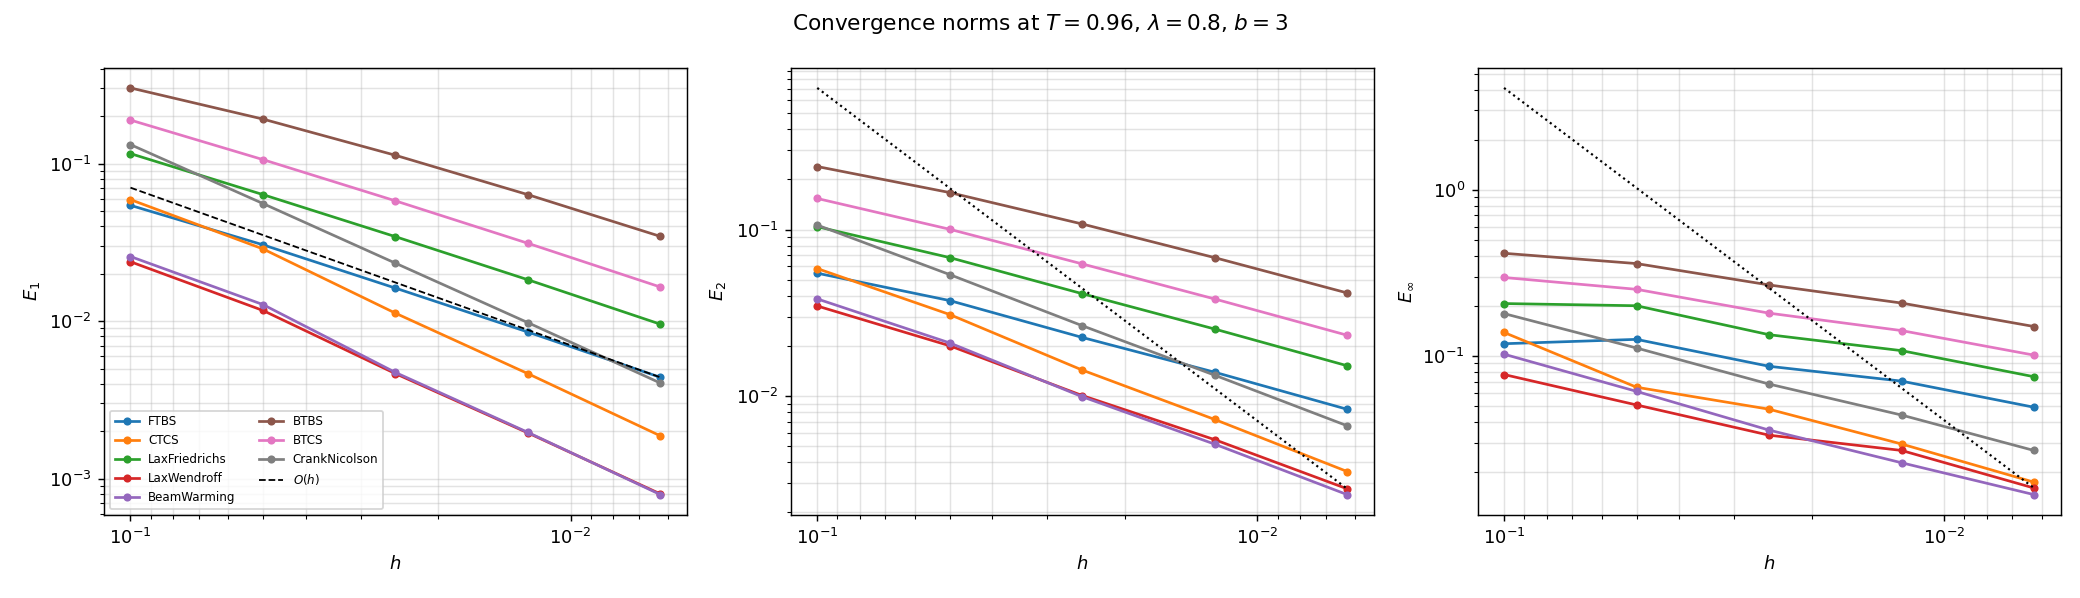
\includegraphics[width=0.97\textwidth]{figures/problem3_convergence_norms.png}
    \end{figure}
    \vspace{-0.15cm}
    \small
    The convergence test uses $T=0.96$, $\lambda=0.8$, $b=3$, and $h=0.1,\ldots,0.00625$.  First-order methods show roughly first-order behavior in $E_1$; formally second-order methods have smaller errors, but the nonsmooth initial corner reduces the observed $E_\infty$ rates.  On the finest grid, representative $E_\infty$ values are about $4.90{\times}10^{-2}$ for FTBS, $1.60{\times}10^{-2}$ for Lax--Wendroff, and $2.69{\times}10^{-2}$ for Crank--Nicolson.
\end{frame}

\begin{frame}{Sweep in $\lambda$: CFL-Limited Explicit Schemes}
    \begin{figure}
        \centering
        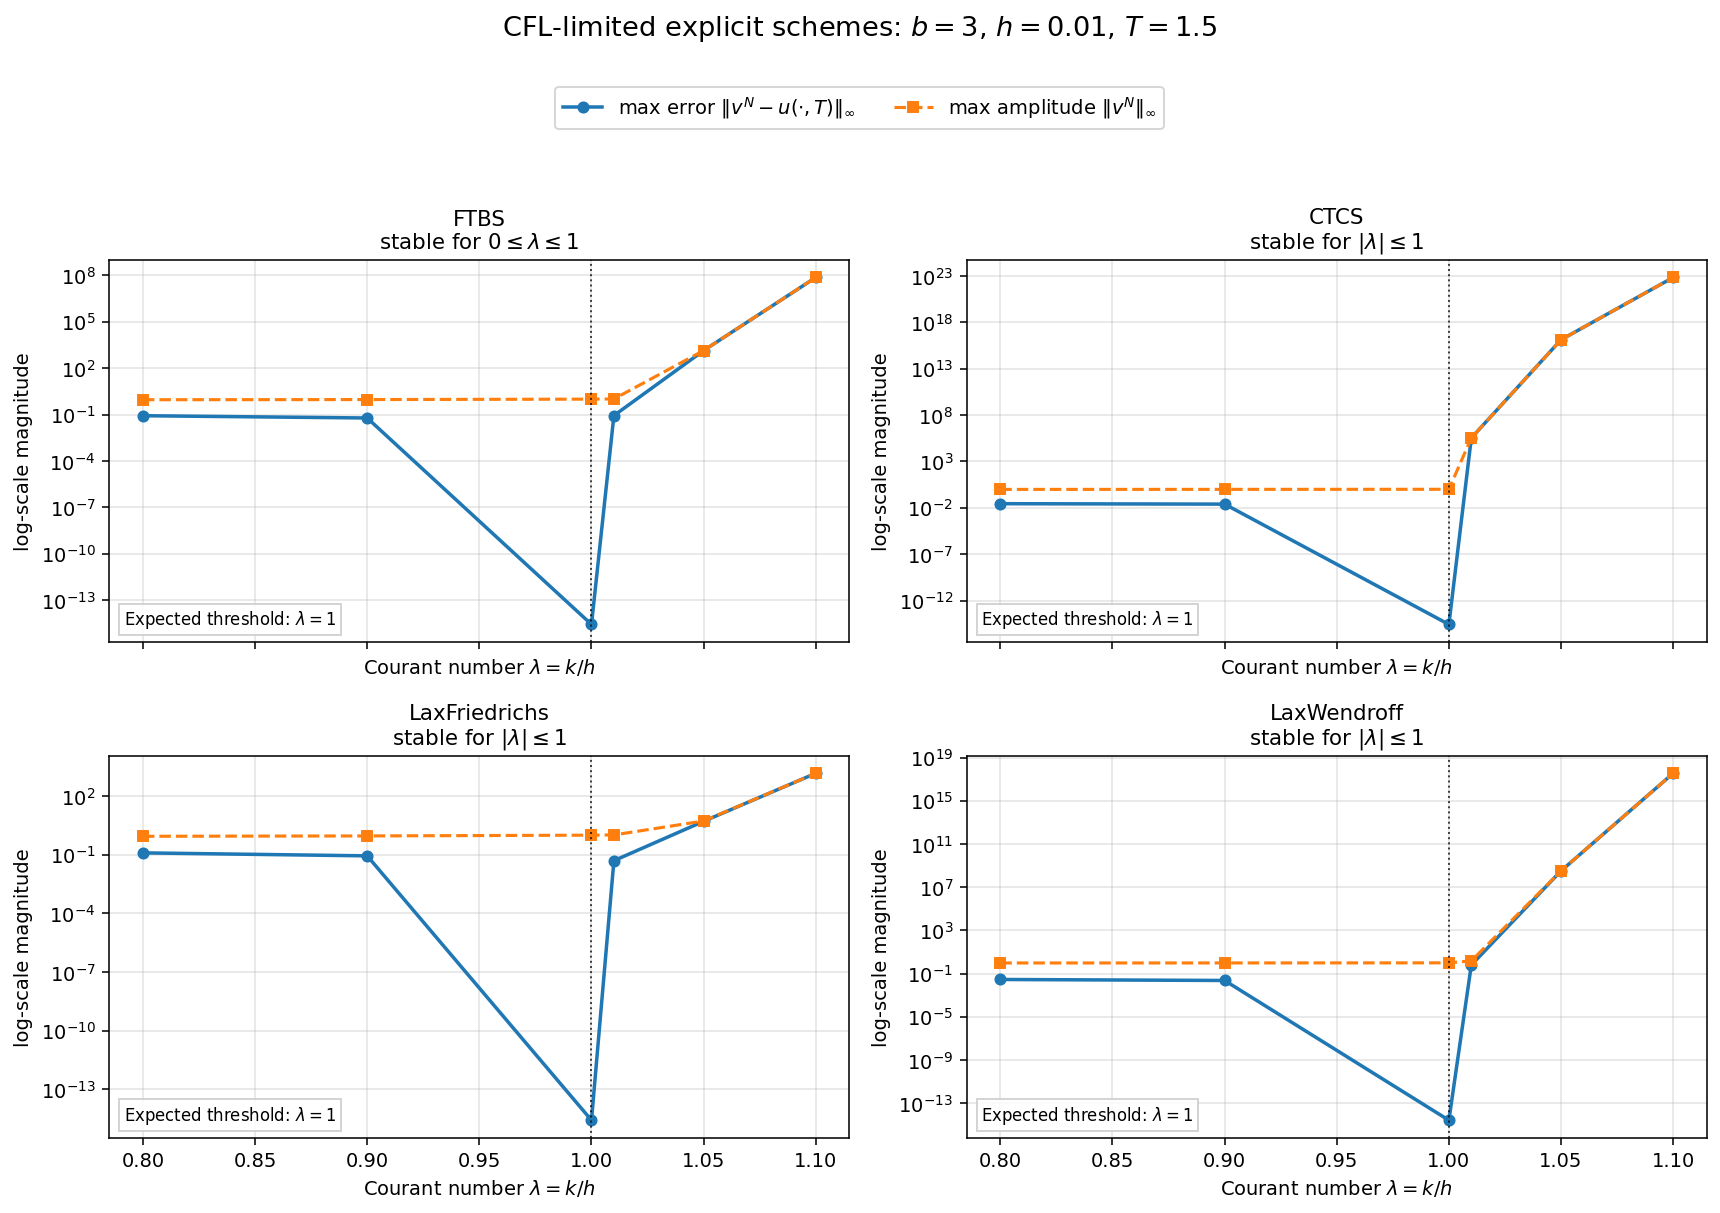
\includegraphics[height=0.64\textheight]{figures/problem3_lambda_sweep_part1_cfl_limited.png}
    \end{figure}
    \vspace{-0.25cm}
    \scriptsize
    These methods are predicted by von Neumann analysis to be stable only up to the
    CFL threshold $\lambda=1$.  At $b=3$, $h=0.01$, and $T=1.5$, the plotted
    quantities are the maximum error $\|v^N-u(\cdot,T)\|_\infty$ and the maximum
    amplitude $\|v^N\|_\infty$.  Once $\lambda$ moves above $1$, the amplitude grows
    rapidly for FTBS, CTCS, Lax--Friedrichs, and Lax--Wendroff, matching the
    theoretical stability boundary.
\end{frame}

\begin{frame}{Sweep in $\lambda$: Unstable and Robust Schemes}
    \begin{figure}
        \centering
        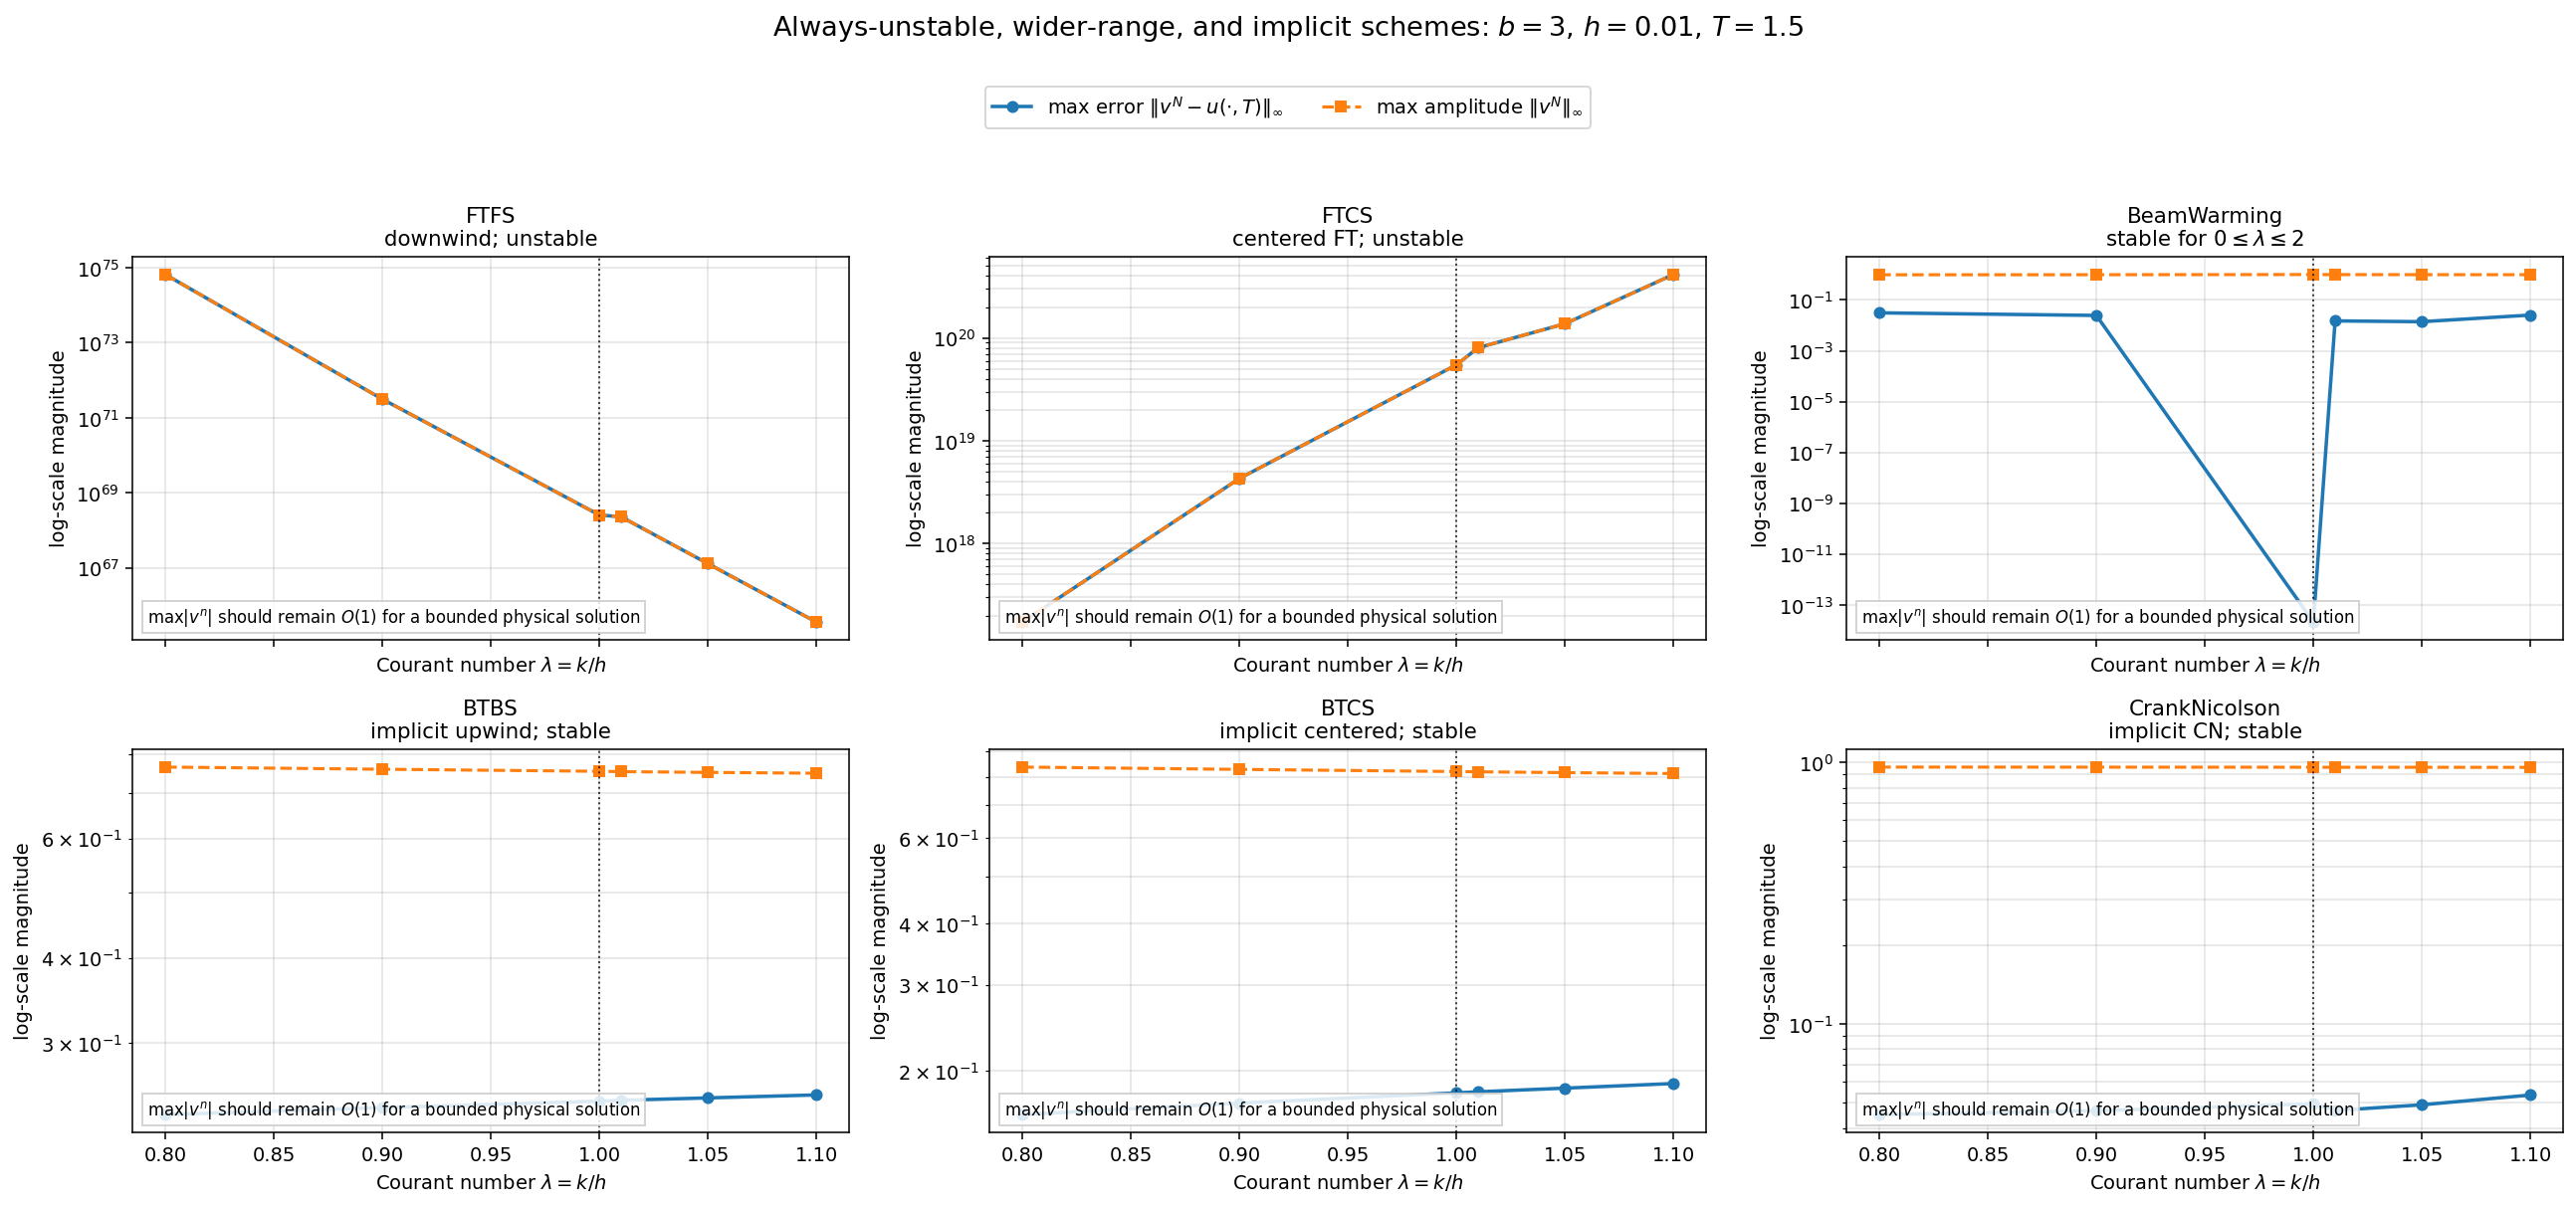
\includegraphics[height=0.62\textheight]{figures/problem3_lambda_sweep_part2_robust_unstable.png}
    \end{figure}
    \vspace{-0.2cm}
    \scriptsize
    FTFS uses the wrong spatial bias for a right-moving wave, and FTCS is unstable
    for pure advection, so both show large amplitudes even when $\lambda<1$.
    Beam--Warming remains bounded for the tested values because its stability range is
    $0\le\lambda\le2$.  The implicit upwind/centered methods, BTBS, BTCS, and
    Crank--Nicolson, also remain bounded as $\lambda$ increases, although BTBS and
    BTCS are visibly more diffusive.
\end{frame}

\begin{frame}{Boundary and Stability Checks}
    \begin{columns}[T]
        \begin{column}{0.48\textwidth}
            \begin{figure}
                \centering
                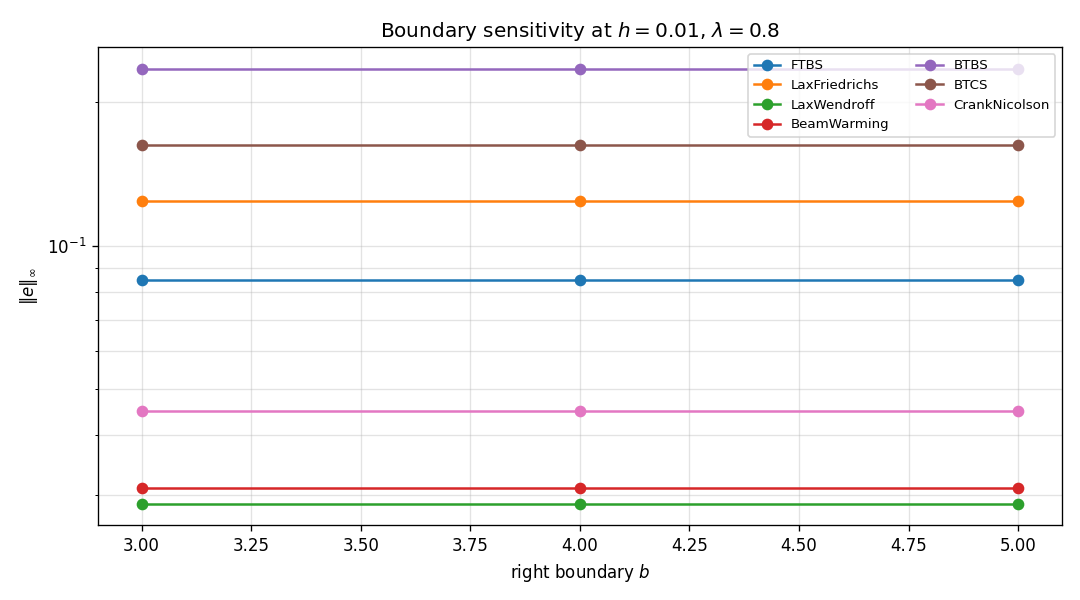
\includegraphics[width=\textwidth]{figures/problem3_boundary_sweep.png}
            \end{figure}
            \scriptsize
            For $T=1.5$, the pulse support is approximately $[0.5,2.5]$, so $b=3$ is already far enough away.  The errors for $b=3,4,5$ coincide.
        \end{column}
        \begin{column}{0.48\textwidth}
            \begin{figure}
                \centering
                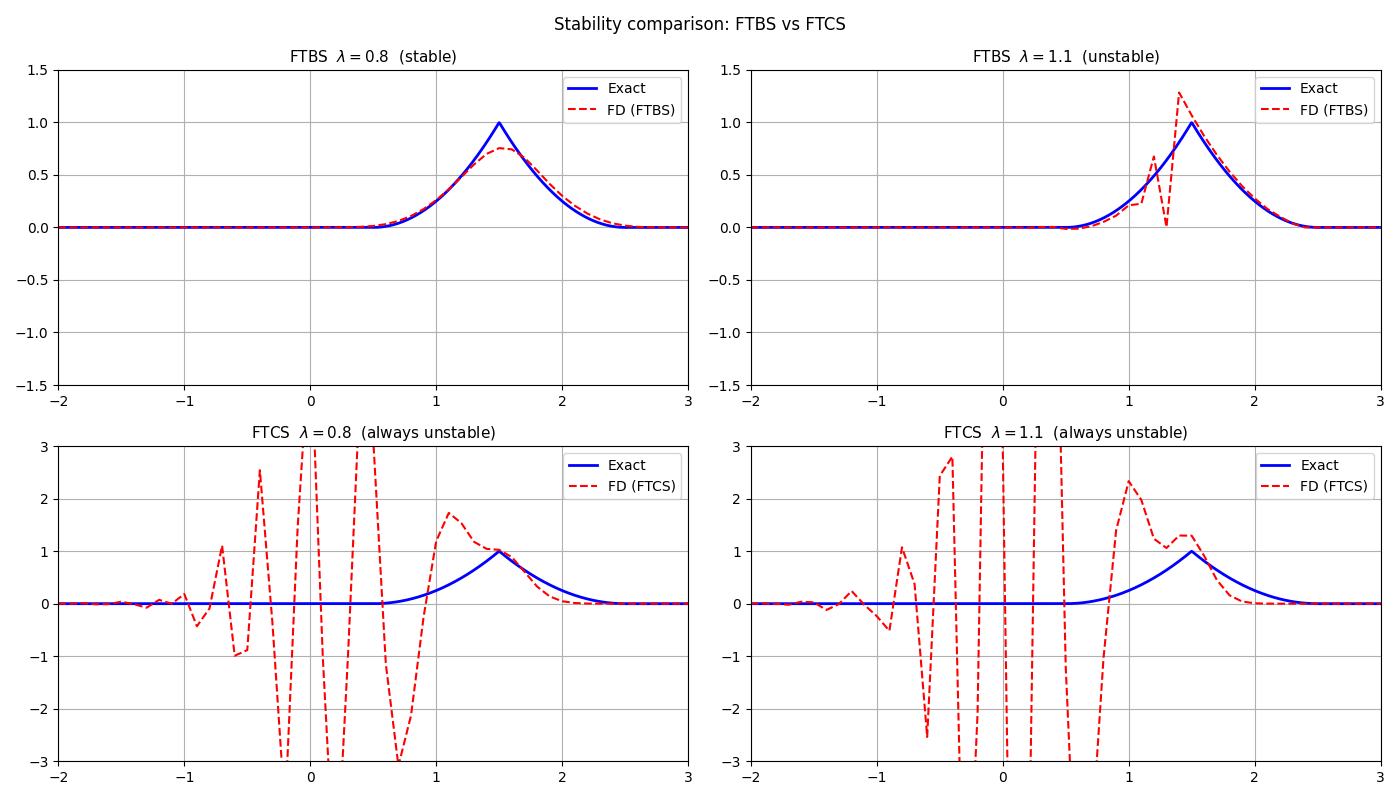
\includegraphics[width=\textwidth]{figures/problem3_stability.png}
            \end{figure}
            \scriptsize
            The direct comparison confirms the theory: FTBS is stable at $\lambda=0.8$ and breaks down above the CFL limit, while FTCS is unstable for advection.
        \end{column}
    \end{columns}
\end{frame}

\begin{frame}{Conclusions}
    \begin{itemize}
        \item The upwind direction matters: for $u_t+u_x=0$, FTBS is the stable explicit upwind method; FTFS is downwind and unstable.
        \item FTCS is unstable for pure advection because $|G|>1$ for nonzero Fourier modes.
        \item Lax--Friedrichs, Lax--Wendroff, and CTCS obey the expected CFL threshold $|\lambda|\le1$.
        \item Beam--Warming remains stable for the tested $\lambda>1$ values, consistent with the wider interval $0\le\lambda\le2$.
        \item BTBS, BTCS, and Crank--Nicolson remain stable as $\lambda$ increases, but stability alone does not imply high accuracy.
        \item The convergence plots agree with the theory after accounting for the nonsmooth corner in $u_0$.
    \end{itemize}
\end{frame}

\end{document}
